\chapter{OOMPH-Lib}
\label{chap:OOMPH-Lib}

\section{Introduction}

This is a parallel library for single or multiple-physics simulation. 
The current version is 0.90. The essential third-party packages that comes with
oomph-lib are:
\begin{enumerate}
  \item BLAS: (non-parallel)
  \item LAPACK: parallel implementation of BLAS, EISPACK, and LINPACK
  \item SuperLU: direct-solver for large, sparse, non-symmetric system of linear
  equations on high-performance machines. It performs LU-decomposition with
  partial pivoting and triangular system CAN BE SOLVED using forward and
  backward substitution.
  \item METIS: a set of serial programs for partitioning finite-element meshes,
  and producing fill reducing ordering for sparse matrices. The algorithms
  implemented here are based on multi-level recursive-bisection, multi-level
  $k$-way, and multi-constraint partitioning schemes.
\end{enumerate}

Also, you may want to include to compile with some third-party libraries
\begin{enumerate}
  \item Hypre 2.0.0: Sect.\ref{sec:hypre}

  \item Trilinos 9.0.2: Object-oriented software framework for the solution of
  large-scale, complex multi-physics engineering
  
\end{enumerate}

Scalability involves architecture of the parallel computer, parallel
implementation of the algorithm, and the scalibility of the algorithm itself.
So, it describes how the system required grows with the size of the problem.

In many large-scale scientific simulation codes, the majority of run times is
spent on linear-solver which solve large, sparse linear systems of equations on
parallel computers.

Prerequisites:
\begin{enumerate}
  \item Install doxygen: 1.8.4
  \item Install Hypre: Sect.\ref{sec:hypre}
  \item Triangle: \url{www.cs.cmu.edu/~quake/triangle.html}, which generate
  exact Delaunay triangulations, Voronoi diagrams, constrained Delaunay
  triangulations, conforming Delaunay triangulations, and high-quality
  triangular meshes. The triangular meshes then can be used for finite-element
  analysis. Compile and add to PATH. 
  \item TetGen: generate tetrahedral meshes of any 3D polyhedral domains.
  Compile and add to PATH.
  \item Modify the files in \verb!external_src/oomph-metis-4.0.0/! by renaming
  \verb!log2! into \verb!log2_function!. This is to avoid the name conflict with
  /usr/include/bits/mathcalls.h:145
\end{enumerate}


How to compile-and-install:
\begin{verbatim}

## Make sure /home/minhtuan/local/hypre/ has 2 subdirs: include, lib
## oomph-lib
mkdir /home/minhtuan/local/oomph-lib
./configure --prefix=/home/minhtuan/local/oomph-lib/ \ 
    --with-hypre=/home/minhtuan/local/hypre/
make --jobs=4 2>&1 | tee m.txt
make install 2>&1 | tee mi.txt
\end{verbatim}

How to link your code to use oomph-lib? Demo codes are provided in
\verb!demo_drivers! folder.
\begin{itemize}
  \item set \verb!LIBDIR! to the /home/minhtuan/local/oomph-lib/lib
  \item add \verb!-LLIBDIR! to the compiler option (to be able to compile the
  code that use the oomph-lib)
  \item add \verb!$LIBDIR! to \verb!LD_RUN_PATH! (to be able to link the
  components) or add any of the following \verb!-Wl, --rpath -Wl, LIBDIR!
  linker flag.
  \item add \verb!$LIBDIR! to the environment variable \verb!LD_LIBRARY_PATH!
  (to be able to run the compiled program)
  \item 
\end{itemize}

\textcolor{red}{How to use it?} - See Sect.\ref{sec:oomph-lib_how2use}.

\textcolor{red}{How to analyze the data?} - The post-processing of oomph-lib
produces ASCII-data in a format that can be read-in by {\bf tecplot} - a commercial plotting
package. We can also use {\bf gnuplot} for simple visualization (not 3D). A
python script written by Angelo Simone can convert the output to VTU format that
can be read by {\bf paraview} (Read visualization book on this section).

\section{Poisson equation}

The Poisson equation is very simple, yet has very powerful applications. Given
the function G, solve for $F$ with the property
\begin{equation}
\Delta F = G
\end{equation}
with $\Delta$ is a symmetric linear operator.

This can be used to \footnote{\url{www.cs.jhu.edu/~misha/Fall07/}} 
\begin{enumerate}
  \item FFT
  \item Jacobi/Gauss-Seidel solvers
  \item Conjugate Gradients
  \item Multigrid
  \item Pre-conditioning
\end{enumerate}

We'll focus on its application in smoothing, i.e. removing artifacts/noise from
surface meshes. Given a function $F:\mathcal{R}^2\rightarrow \mathcal{R}$, the
{\bf gradient of F} is the vector field $\nabla F: \mathcal{R}^2 \rightarrow\mathcal{R}^2$ 
defined as the partial derivatives
\begin{equation}
\nabla F(x,y) = \left( \frac{\partial F}{\partial x}, \frac{\partial
F}{\partial y}\right)
\end{equation}
So, at the point $p_o$, the vector $\nabla F(p_o)$ points in the direction of
greatest change of $F$, Fig.\ref{fig:gradient}.


\begin{figure}[hbt]
  \centerline{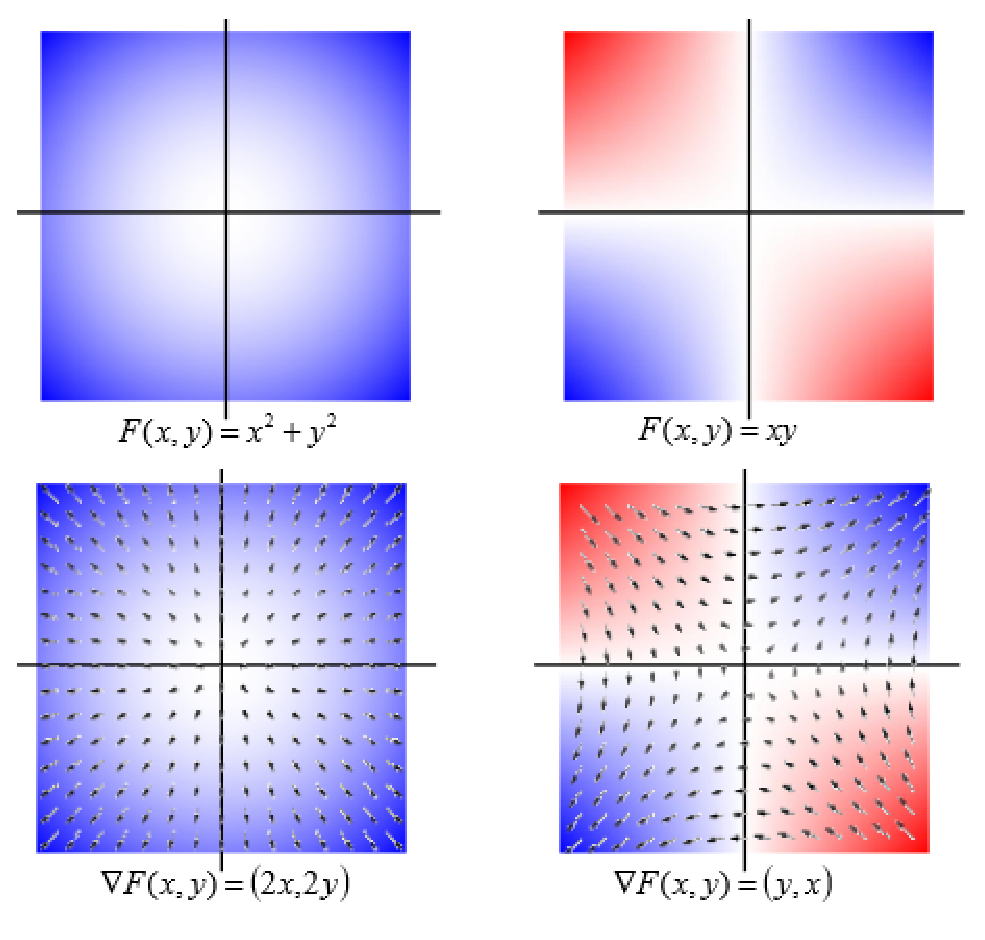
\includegraphics[height=4cm,
    angle=0]{./images/gradient.eps}}
  \caption{The vector fields}
\label{fig:gradient}
\end{figure}

The set of all gradients is called the vector field. Given a vector field
$\vec{F}=(F_1,F_2): \mathcal{R}^2\rightarrow \mathcal{R}^2$, the {\bf divergence
of $\vec{F}$} is the function: $\nabla \cdot \vec{F}: \mathcal{R}^2\rightarrow
\mathcal{R}$, defined by the partial derivatives
\begin{equation}
\nabla \cdot \vec{F}(x,y) = \frac{\partial F_1}{\partial x} + \frac{\partial
F_2}{\partial y}
\end{equation}
So, at the point $p_o$, the divergence $\nabla\cdot F(p_o)$ is a measure of the
extent to which the flow (de)compresses at $p_o$.

{\bf The Laplacian of F} is the function $\Delta F: \mathcal{R}^2\rightarrow
\mathcal{R}$ (or $\nabla^2F$)
\begin{equation}
\Delta F(x,y) = \nabla\cdot\left(\nabla F(x,y) \right) = \frac{\partial^2
F}{\partial x^2} + \frac{\partial^2 F}{\partial y^2}
\end{equation}
So, at the point $p_o$, the Laplacian of F measures the extent to which the
value of F at $p_o$ differs from the average value of $F$ of its neighbors.  

The Laplacian of F can be defined by considering the family of smoothed
functions
\begin{equation}
G(t,x,y) = F(x,y)\star e^{-\left(x^2+y^2\right)/t}
\end{equation}
which satisfies the property: 
\begin{equation}
\frac{\partial G}{\partial t}|_{t=0}=\Delta F
\end{equation}

The function F can be updated to perform a small amount of function smoothing on
the function F
\begin{equation}
F(x,y) \leftarrow F(x,y) + \varepsilon \Delta F(x,y)
\end{equation}





\section{Using oomph-lib}
\label{sec:oomph-lib_how2use}

We define the problem as an object, and then call the appropriate solver. By
default, the problem is assumed to be non-linear and the Newton's method is used
(using Jacobian matrix).

\begin{verbatim}
 main()
        {
          // Create the problem object
          MyProblem problem; 
          
          // Solve the problem, using oomph-lib's default Newton solver
          problem.newton_solve();
        }
\end{verbatim}
The problem is an instance of the {\bf MyProblem} class. So, basically, you need
to write your own class, say MyProblem, which is an inheritance from the generic
{\bf oomph::Problem} class. How much effort to write your own class depends on
the problem. A few member functions need to be implemented
\begin{enumerate}
  \item \verb!MyProblem()!: the constructor
  \item \verb!Problem::actions_before_newton_solve()! and 
\verb!Problem::actions_after_newton_solve()!: two member functions 
\end{enumerate}

To write the constructor, we need to tell
\begin{enumerate}
  \item the time-step: 
  \begin{verbatim}
  Problem::add_time_stepper_pt(new SomeTimeStepper());
  \end{verbatim}
 \item the {\bf Mesh} object (for finite-element simulation):
 Sect.\ref{sec:oomph_mesh}
 \begin{verbatim}
 Problem::mesh_pt() = new SomeMesh<SomeElement>(...);
 \end{verbatim}
 
 \item the boundary condition: (by default) all nodal values are assumed to be
 free and be zero initially. So, for those that are boundary values and/or
 initial values are not zero, then we need to set. For example: node 0 is the
 boundary and is always to be 10, then we 'pin' a value 10 to it
 \begin{verbatim}
 Problem::mesh_pt()->node_pt(0)->pin(0);
 
 // Set the first element (0,) to value 1.0
 Problem::mesh_pt()->node_pt(0)->set_value(0,1.0);
 \end{verbatim}
 NOTE: \textcolor{red}{The first element is zero-th index based on C++
 indexing scheme.}
 
 \item 
\end{enumerate}

and is treated as a set of algebraic
equations of unknown {\bf u} and the parameters $\mathbf{\lambda}$:
$\mathbf{R(u,\lambda)}=0)$.

\subsection{Documentation}

OOMPH-Lib comes with \verb!DocInfo! class which uses ifstream and ofstream to
test if folder for writing exists. However, in BG/Q it doesn't work, then we can
derive a new class which contais the data member to keep the folder name
\verb!Folder!, and the 
\begin{lstlisting}
//cardiac_utilities.h
class CardiacDocInfo
{

private:
  std::string Folder;
  unsigned Number;
public:

  CardiacDocInfo();

  void set_directory(std::string folder);

  std::string& directory();

  unsigned& number();

};
\end{lstlisting}




\subsection{Build Mesh}
\label{sec:oomph_mesh}

\subsection{Example: Poisson 1D}

Poisson problem or Poisson equation has a very broad range of applications in
mechanical engineering, electrostatics, etc. It's a PDE of elliptic type, with
the general form which arises in steady-state heat conduction with distributed
source $\phi$ (temperature), and $\phi(x,y)$ is the stress function:
\begin{equation}
\nabla^2\phi + g = 0
\end{equation}

Example 1:
\begin{equation}
\frac{\partial^2 u}{\partial x^2} = \pm 30\sin(\sqrt{3x})
\end{equation}
with $x\in [0,1]$, and boundary conditions $u(0)=1, u(1)=\mp 1$

Another example is
\begin{equation}
\frac{\partial^2 u}{\partial x^2}= s(x) = 4\pi^2.\sin(\pi x).\cos(\pi x)
\end{equation}
with $x\in [0,1]$, and boundary condition $u(0)=u(1)=0$.

Now, how to represent the PDE as a \verb!Problem! object.
